\documentclass{ximera}
\graphicspath{     %% setup a global graphics path
{./}               %% look in the same-level directory
{./pictures/}      %% look in graphics
{../pictures/}     %% look up one directory, then in graphics
%{../../pictures/} %% look up two directories, then in graphics
}

\author{Zack Reed}
%borrowed from selinger linear algebra
\begin{document}

\begin{problem}\label{prob:proj1a}
  If $\vec{d}=\begin{bmatrix}-1\\3\end{bmatrix}$ and $\vec{v}=\begin{bmatrix}1\\4\end{bmatrix}$ then
  $$\mbox{proj}_{\vec{d}}\vec{v}=\begin{bmatrix}\answer{-1.1}\\\answer{3.3}\end{bmatrix}$$
    \end{problem}
     
    \begin{problem}\label{prob:proj1b}
    If $\vec{d}=\begin{bmatrix}0\\2\\1\end{bmatrix}$ and $\vec{v}=\begin{bmatrix}-1\\-4\\2\end{bmatrix}$ then
    $$\mbox{proj}_{\vec{d}}\vec{v}=\begin{bmatrix}\answer{0}\\\answer{-2.4}\\\answer{-1.2}\end{bmatrix}$$
    \end{problem}
 
\begin{problem}\label{prob:proj2}
Find the projection of vector $\vec{v}$ onto line $l$. (If entering answers in decimal form, round to the nearest one hundredth.)
 
\begin{center}
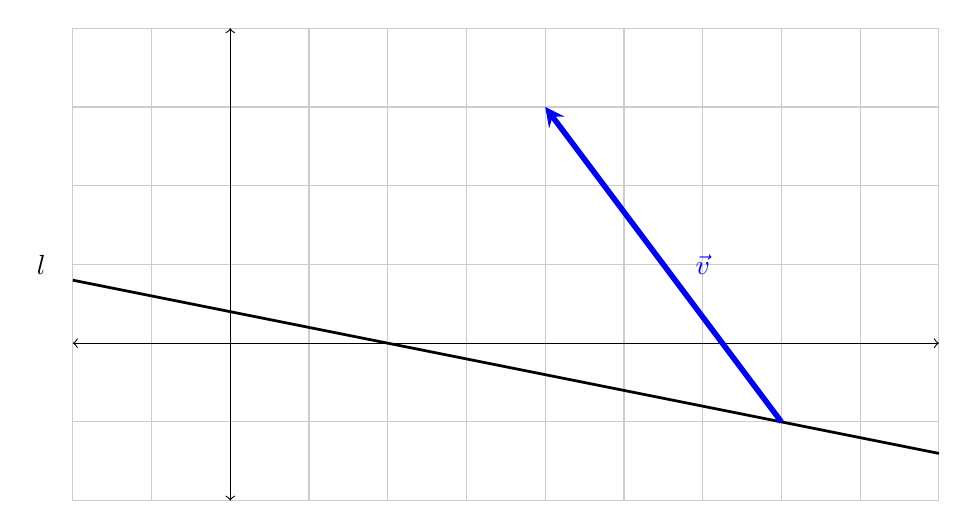
\begin{tikzpicture}
\draw[thin,gray!40] (-2,-2) grid (9,4);
  \draw[<->] (-2,0)--(9,0);
  \draw[<->] (0,-2)--(0,4);
  \node[blue] at (6, 1)   (a) {$\vec{v}$};
  \node[] at (-2.4, 1)   (b) {$l$};
  \draw [-,line width=1pt]  (-2,0.8)--(9, -1.4);
\draw[line width=2pt,blue,-stealth](7, -1)--(4,3);
\end{tikzpicture}
\end{center}
 
Answer:
$$\begin{bmatrix}\answer[tolerance=0.005]{-95/26}\\\answer[tolerance=0.005]{19/26}\end{bmatrix}$$
\end{problem}
 
\begin{problem}\label{prob:distpttoline}
Find the distance between point $A$ and line $l$.
 
\begin{center}
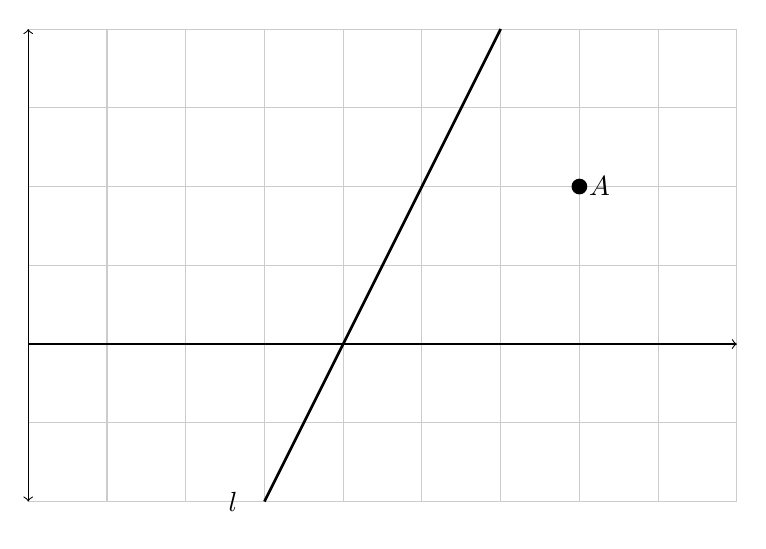
\begin{tikzpicture}
\draw[thin,gray!40] (0,-2) grid (9,4);
  \draw[->] (0,0)--(9,0);
  \draw[<->] (0,-2)--(0,4);
  \fill (7,2)node[above, right]{$A$} circle (1mm);
  \node[] at (2.6, -2)   (b) {$l$};
  \draw [-,line width=1pt]  (3,-2)--(6, 4);
\end{tikzpicture}
\end{center}
 
Answer: $\sqrt{\answer{3.2}}$.
\end{problem}
 
\begin{problem}\label{prob:circletangenttoline}
Find the radius of a circle centered at $(4, 2)$ if the line $y=\frac{3}{2}x+3$ is tangent to the circle.  Enter your response as a fraction.
 
Answer:
$$r=\sqrt{\answer{196/13}}$$
The graph below shows the line $y=\frac{3}{2}x+3$ together with a circle of radius $1$.  Change the value of $r$ to the radius you have found to visualize the correct answer.
 
 
 
 
\end{problem}


\end{document}